\section{Pairwise clustering}

\mode<presentation>{
\begin{frame} 
    \begin{center} \huge
        \secname
    \end{center}
    \begin{itemize}
		\item Proximity to $\underset{\text{other points}}{\cancel{\text{prototype}}}$
		\item A proper application of mean-field annealing
		\item A building block for ``soft'' K-means
    \end{itemize}
\end{frame}
}


\begin{frame}{Notions of proximity}

\textbf{Recall} that K-means clusters points based on their proximity to some prototype.\\

\svspace{-4mm}

\begin{center}
	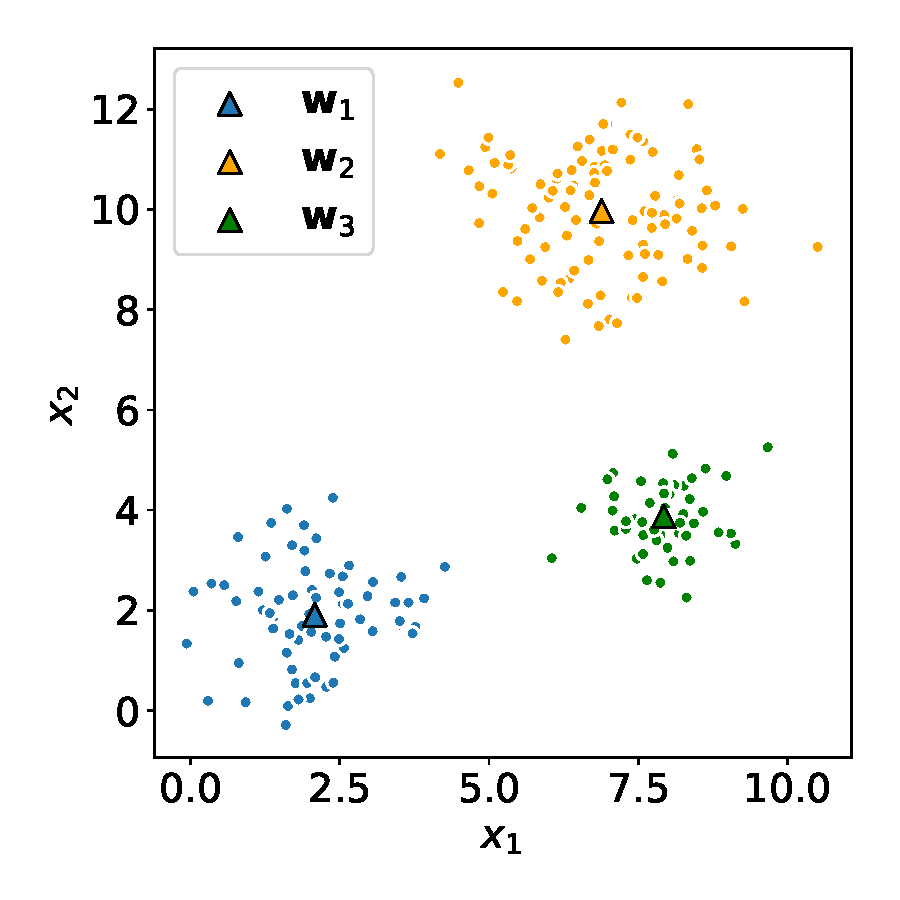
\includegraphics[width=0.35\textwidth]{img/m3_data}
	\notesonly{
	\captionof{figure}{2D data with M=3 prototypes}
	}
\end{center}
\begin{center}
	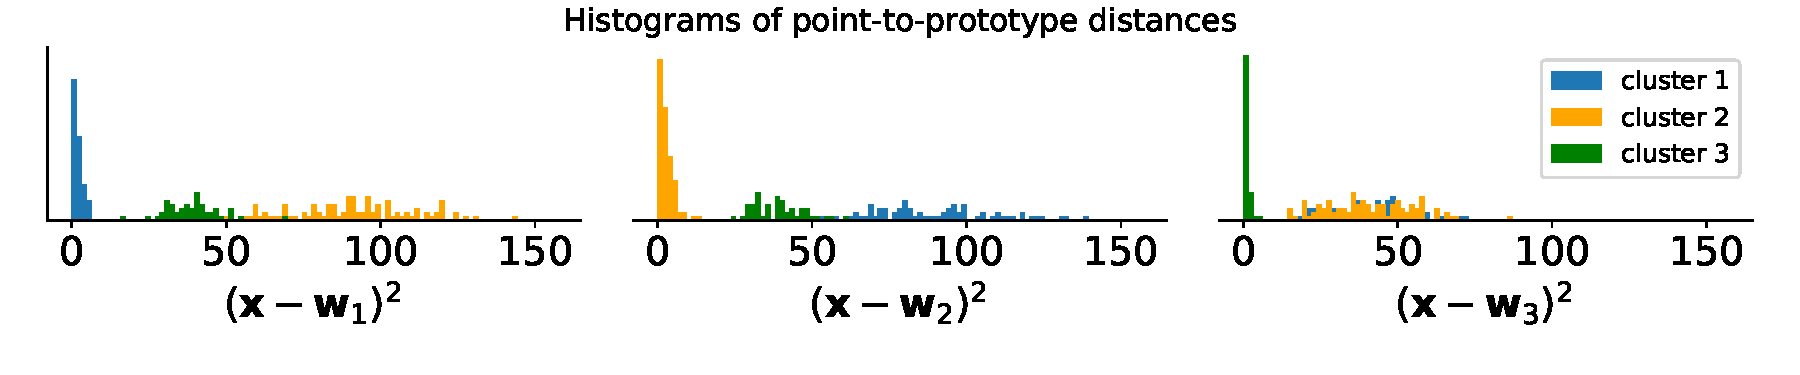
\includegraphics[width=0.95\textwidth]{img/m3_hist_point_proto} 
	\notesonly{
	\captionof{figure}{Proximity to M=3 prototypes}
	}
\end{center}

\end{frame}

\begin{frame}{Notions of proximity: pairwise distance}

\begin{center}
\begin{minipage}{0.32\textwidth}
	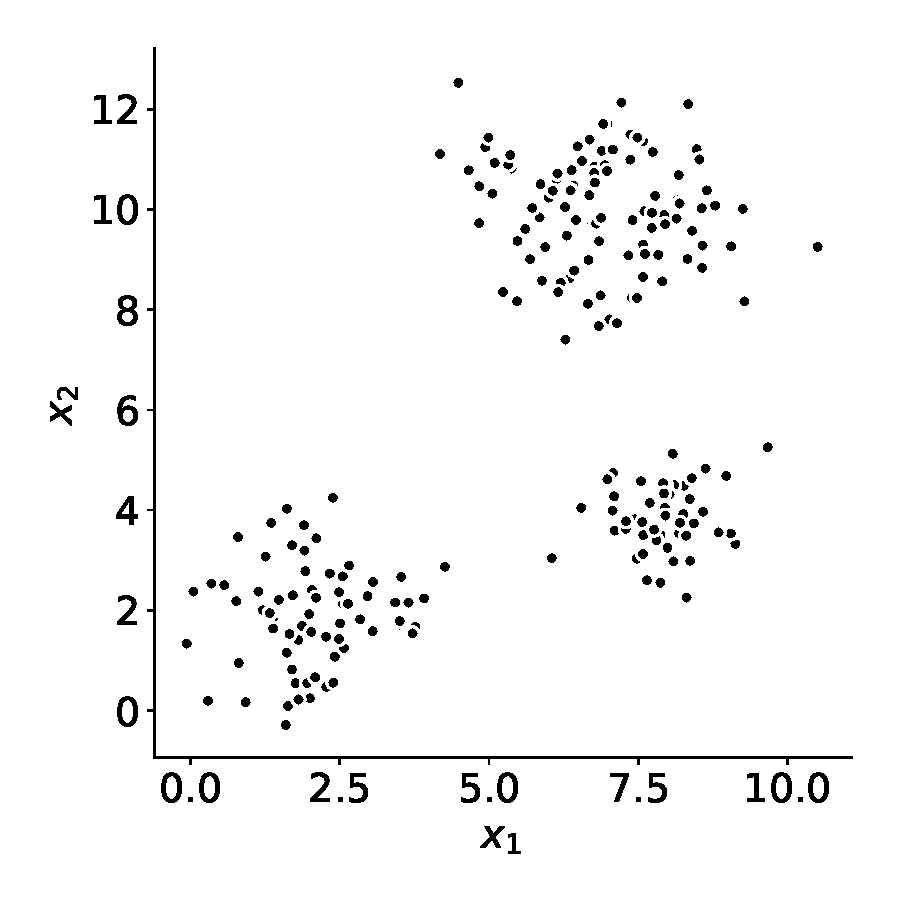
\includegraphics[width=0.85\textwidth]{img/m3_data_nocolor} 
\end{minipage}
\begin{minipage}{0.32\textwidth}
	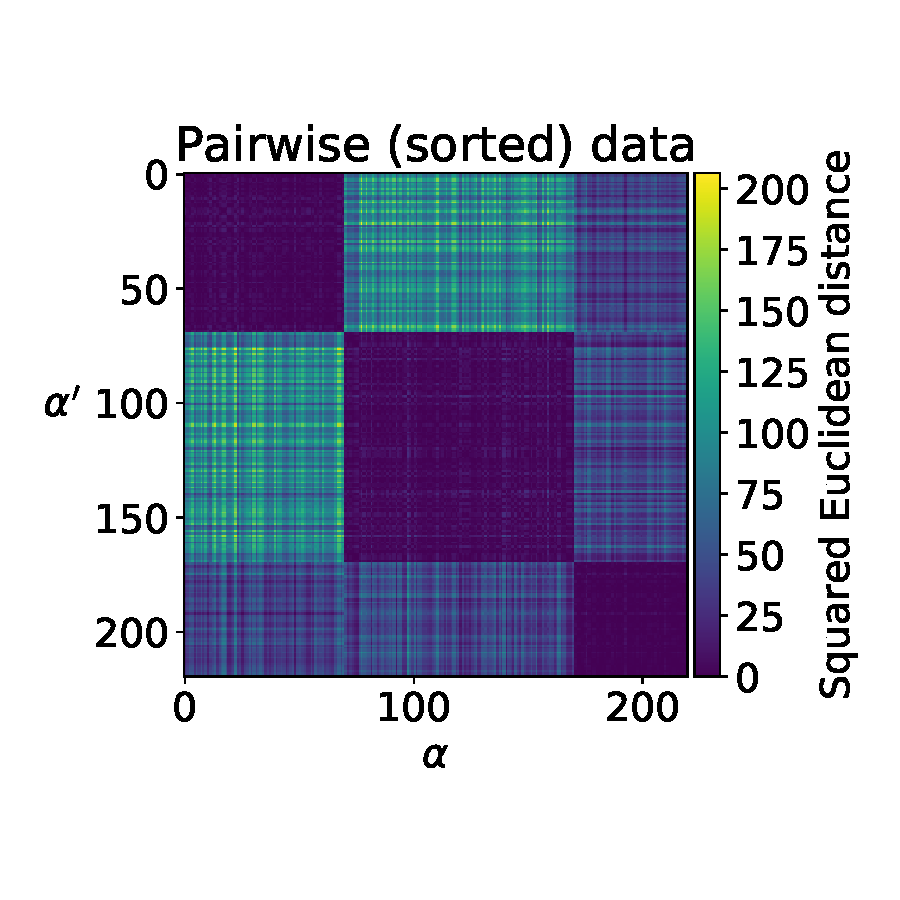
\includegraphics[width=0.99\textwidth]{img/m3_pdist} 
\end{minipage}
\begin{minipage}{0.32\textwidth}
	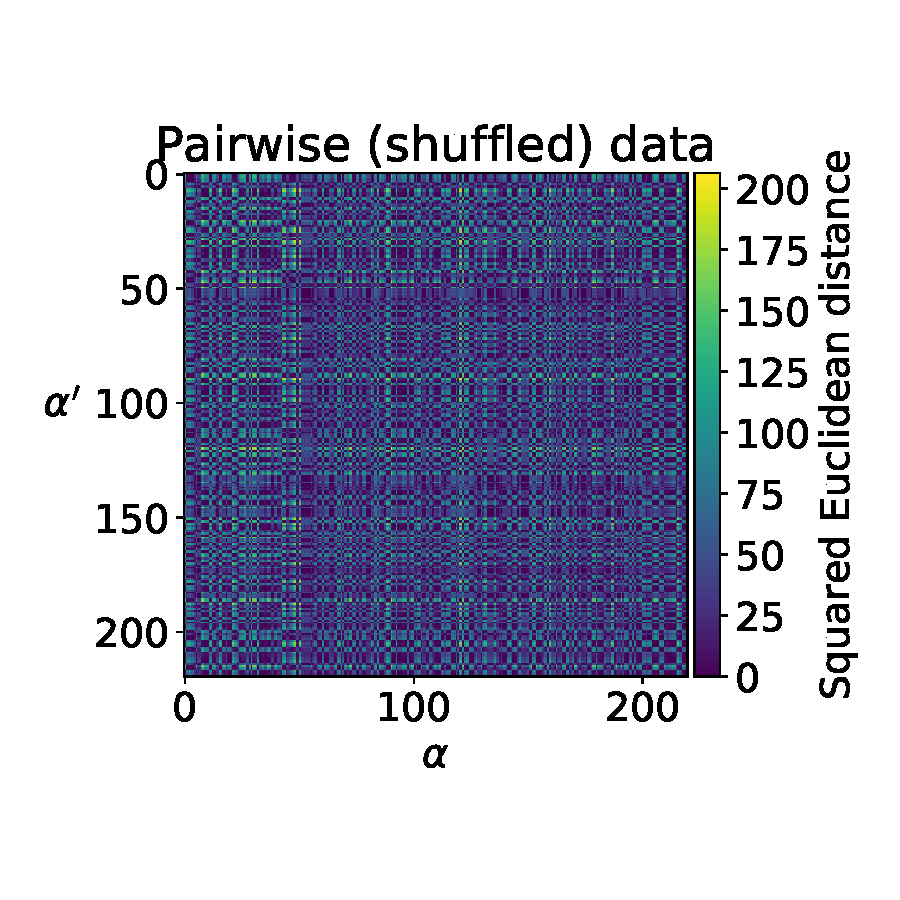
\includegraphics[width=0.99\textwidth]{img/m3_pdist_shuffled} 
\end{minipage}
	\notesonly{
	\captionof{figure}{Pairwise distances. The points were sorted by cluster to highlight the box-structure in the pairwise distances. This is purely for visualization purposes. Pairwise clustering does not require any prior sorting of the data.}
	}
\end{center}

\notesonly{
Another approach to describing a similar ``structure'' in the data
can be based on the following:}
%\slidesonly{
%\begin{figure}[h!]
  %\centering
%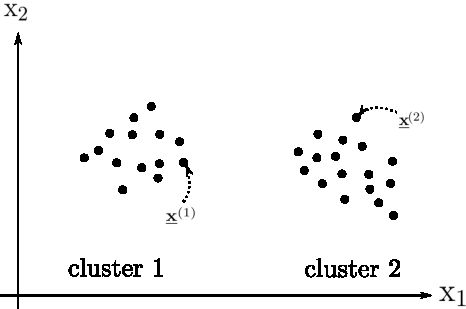
\includegraphics[height=3cm]{img/clustering} 
%\end{figure}

When we reason about structure in the data:\\
%}
Points that are ``close'' to one another have more in common than points that are far away from one another. 
\notesonly{
We cluster points based on their \emph{proximity to one another}. 
A point that is further away from this collection is grouped with other points that are closer to it. Pairwise clustering is about grouping points based on their pairwise relations. \\
}
We will first discuss clustering based on \emph{pairwise distances} and eventually extend this to \emph{soft clustering}.

\end{frame}

